
\section{Velocity \textit{vs.}~Time Graphs\footnote{
1990-93 Dept. of Physics and Astronomy, Dickinson College. Supported by FIPSE
(U.S. Dept. of Ed.) and NSF. Portions of this material may have been modified
locally and may not have been classroom tested at Dickinson College.
}}

\makelabheader %(Space for student name, etc., defined in master.tex or labmanual_formatting_commands.tex)

\bigskip

\textbf{Objectives }

\begin{itemize}[nosep]
\item To acquire an intuitive understanding of speed and velocity in one dimension. 
\item To learn how to relate graphs of velocity \textit{vs.}~time to the motions they represent.
\end{itemize}

\bigskip
\textbf{Apparatus}

\begin{itemize}[nosep]
\item \textit{Capstone} software (\filename{V\_Graphs.cap} experiment file)
\item Wireless motion sensor
\item Wooden board
\end{itemize}

\bigskip
\textbf{Introduction} 

You have already plotted your position as a function of time. Another way to
represent your motion during an interval of time is with a graph which describes
how fast and in what direction you are moving from moment to moment. How fast
you move is known as your speed. Velocity is a quantity which takes into account your speed and the direction you are moving. It is the rate of change of position with respect
to time. Thus, when you examine the motion of an object moving
along a line, its velocity can be positive or negative depending
on whether the object is moving in the positive or negative direction.

Graphs of velocity over time are more challenging to create and interpret than
those for position. A good way to learn to interpret them is to create and examine velocity \textit{vs.}~time graphs of your own body motions, as you will do in the next few activities.

\bigskip

\textbf{Activity 1: Making Velocity \textit{vs.}~Time Graphs} 

To make the graphs in the following activities, open the \filename{V\_Graphs.cap} application in the \filename{\coursefolder} folder. Turn on the sensor at your station. To connect it to the computer via Bluetooth, select \textbf{Hardware Setup} and select the correct address that matches its Device ID Number (XXX-XXX). To start a data run, click the \textbf{Record} button. To stop a data run, click the \textbf{Stop} button.

(a) Make a velocity graph by walking away from the sensor slowly and steadily.
Try again until you get a graph you're satisfied with and then sketch your result
on the graph that follows. (We suggest you draw smooth patterns by ignoring
smaller bumps that are mostly due to your steps.)

%\vspace{0.3cm}
%{\par\centering 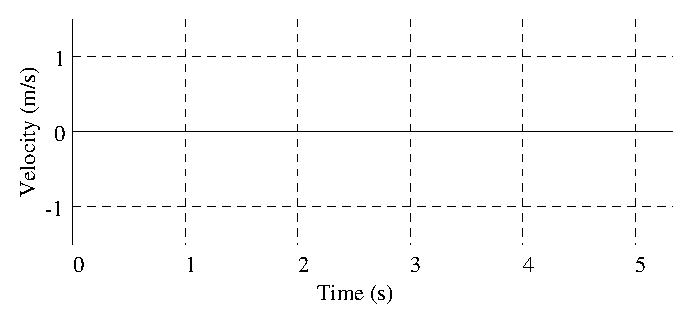
\includegraphics{velocity/velocity_fig1.eps} \par}
%\vspace{0.3cm}
\begin{lab_axis}*[lab_grid,
	width=4.5in, height=1.8in,
	xlabel={Time (s)},
	ylabel={Velocity (m/s)},
	xmin=0, xmax=5,
	ymin=-2, ymax=2,
	xtick distance = 1,
	ytick distance = 1,
	minor x tick num=1,
	]
\end{lab_axis}

(b) Make a velocity graph, walking away from the sensor steadily at a medium
speed. Sketch your graph below.

%\vspace{0.3cm}
%{\par\centering 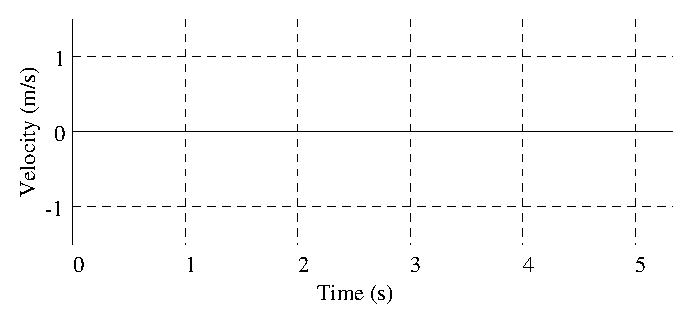
\includegraphics[width=0.7\textwidth]{velocity/velocity_fig1.eps} \par}
%\vspace{0.3cm}
\begin{lab_axis}*[lab_grid,
	width=4.5in, height=1.8in,
	xlabel={Time (s)},
	ylabel={Velocity (m/s)},
	xmin=0, xmax=5,
	ymin=-2, ymax=2,
	xtick distance = 1,
	ytick distance = 1,
	minor x tick num=1,
	]
\end{lab_axis}

(c) Make a velocity graph, walking toward the sensor slowly and steadily.
Sketch your graph below.

%\vspace{0.3cm}
%{\par\centering 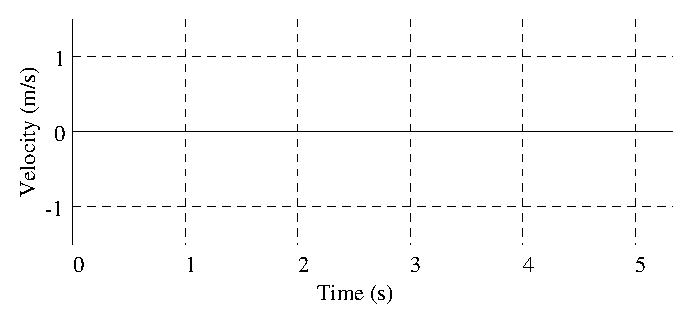
\includegraphics[width=0.7\textwidth]{velocity/velocity_fig1.eps} \par}
%\vspace{0.3cm}
\begin{lab_axis}*[lab_grid,
	width=4.5in, height=1.8in,
	xlabel={Time (s)},
	ylabel={Velocity (m/s)},
	xmin=0, xmax=5,
	ymin=-2, ymax=2,
	xtick distance = 1,
	ytick distance = 1,
	minor x tick num=1,
	]
\end{lab_axis}

(d) What is the most important difference between the graph made by slowly walking
away from the sensor and the one made by walking away more quickly? 
\answerspace{25mm}

(e) How are the velocity \textit{vs.}~time graphs different for motion away and motion
toward the sensor?
\answerspace{25mm}

\pagebreak[2]
\textbf{Activity 2: Predicting a Velocity \textit{vs.}~Time Graph }

Suppose you were to undergo the following sequence of motions: (1) walk away
from the sensor slowly and steadily for 6 seconds, (2) stand still for 6 seconds,
(3) walk toward the sensor steadily about twice as fast as before.

(a) Use a dashed line in the graph that follows to record your prediction of
the shape of the velocity graph that will result from the motion described above.

%\vspace{0.3cm}
%{\par\centering 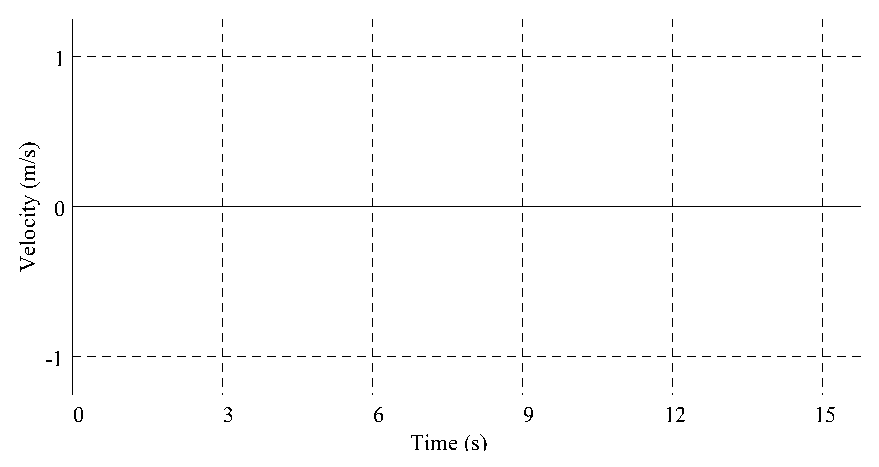
\includegraphics[width=0.7\textwidth]{velocity/velocity_fig2.eps} \par}
%\vspace{0.3cm}
\begin{lab_axis}*[lab_grid,
	width=4.5in, height=1.8in,
	xlabel={Time (s)},
	ylabel={Velocity (m/s)},
	xmin=0, xmax=20,
	ymin=-2, ymax=2,
	xtick distance = 4,
	ytick distance = 1,
	minor x tick num=1,
	]
\end{lab_axis}

(b) Compare predictions with your partner(s) and see if you can all agree. Use
a solid line to sketch your group prediction in the graph above.

(c) Adjust the sampling time to 15 s and then test your prediction. Repeat your
motion until you are confident that it matches the description in words and
then draw the actual graph on the axes below. Be sure the 6-second stop shows
clearly.

%\vspace{0.3cm}
%{\par\centering 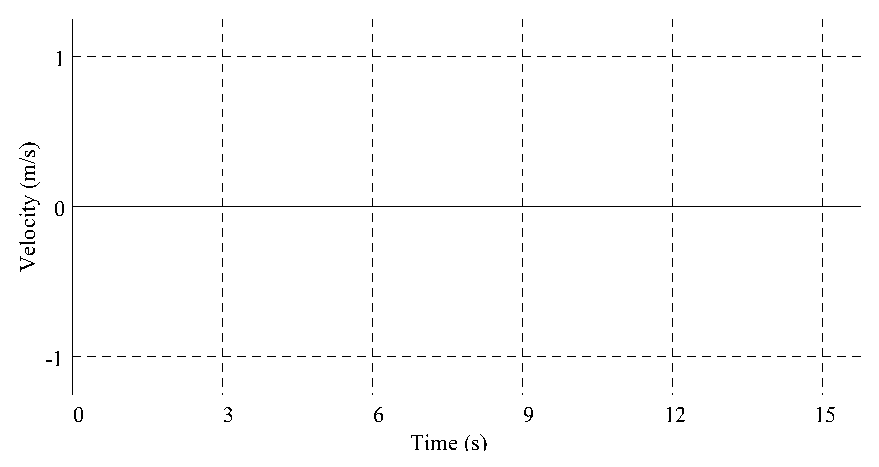
\includegraphics[width=0.7\textwidth]{velocity/velocity_fig2.eps} \par}
%\vspace{0.3cm}
\begin{lab_axis}*[lab_grid,
	width=4.5in, height=1.8in,
	xlabel={Time (s)},
	ylabel={Velocity (m/s)},
	xmin=0, xmax=20,
	ymin=-2, ymax=2,
	xtick distance = 4,
	ytick distance = 1,
	minor x tick num=1,
	]
\end{lab_axis}

(d) Did your prediction match your real motion? If not, what misunderstanding
of what elements of the graph did you have?
\answerspace{20mm}

\pagebreak[2]
\textbf{Velocity Vectors} 

The two ideas of speed and direction can be combined and represented by vectors.
A velocity vector is represented by an arrow pointing in the direction of motion.
The length of the arrow is drawn proportional to the speed; the longer the arrow,
the larger the speed. If you are moving toward the right, your velocity vector
can be represented by the arrow shown below.

\vspace{0.3cm}
%{\par\centering 
\includegraphics{velocity/velocity_fig3.eps} \par}
{\par\centering 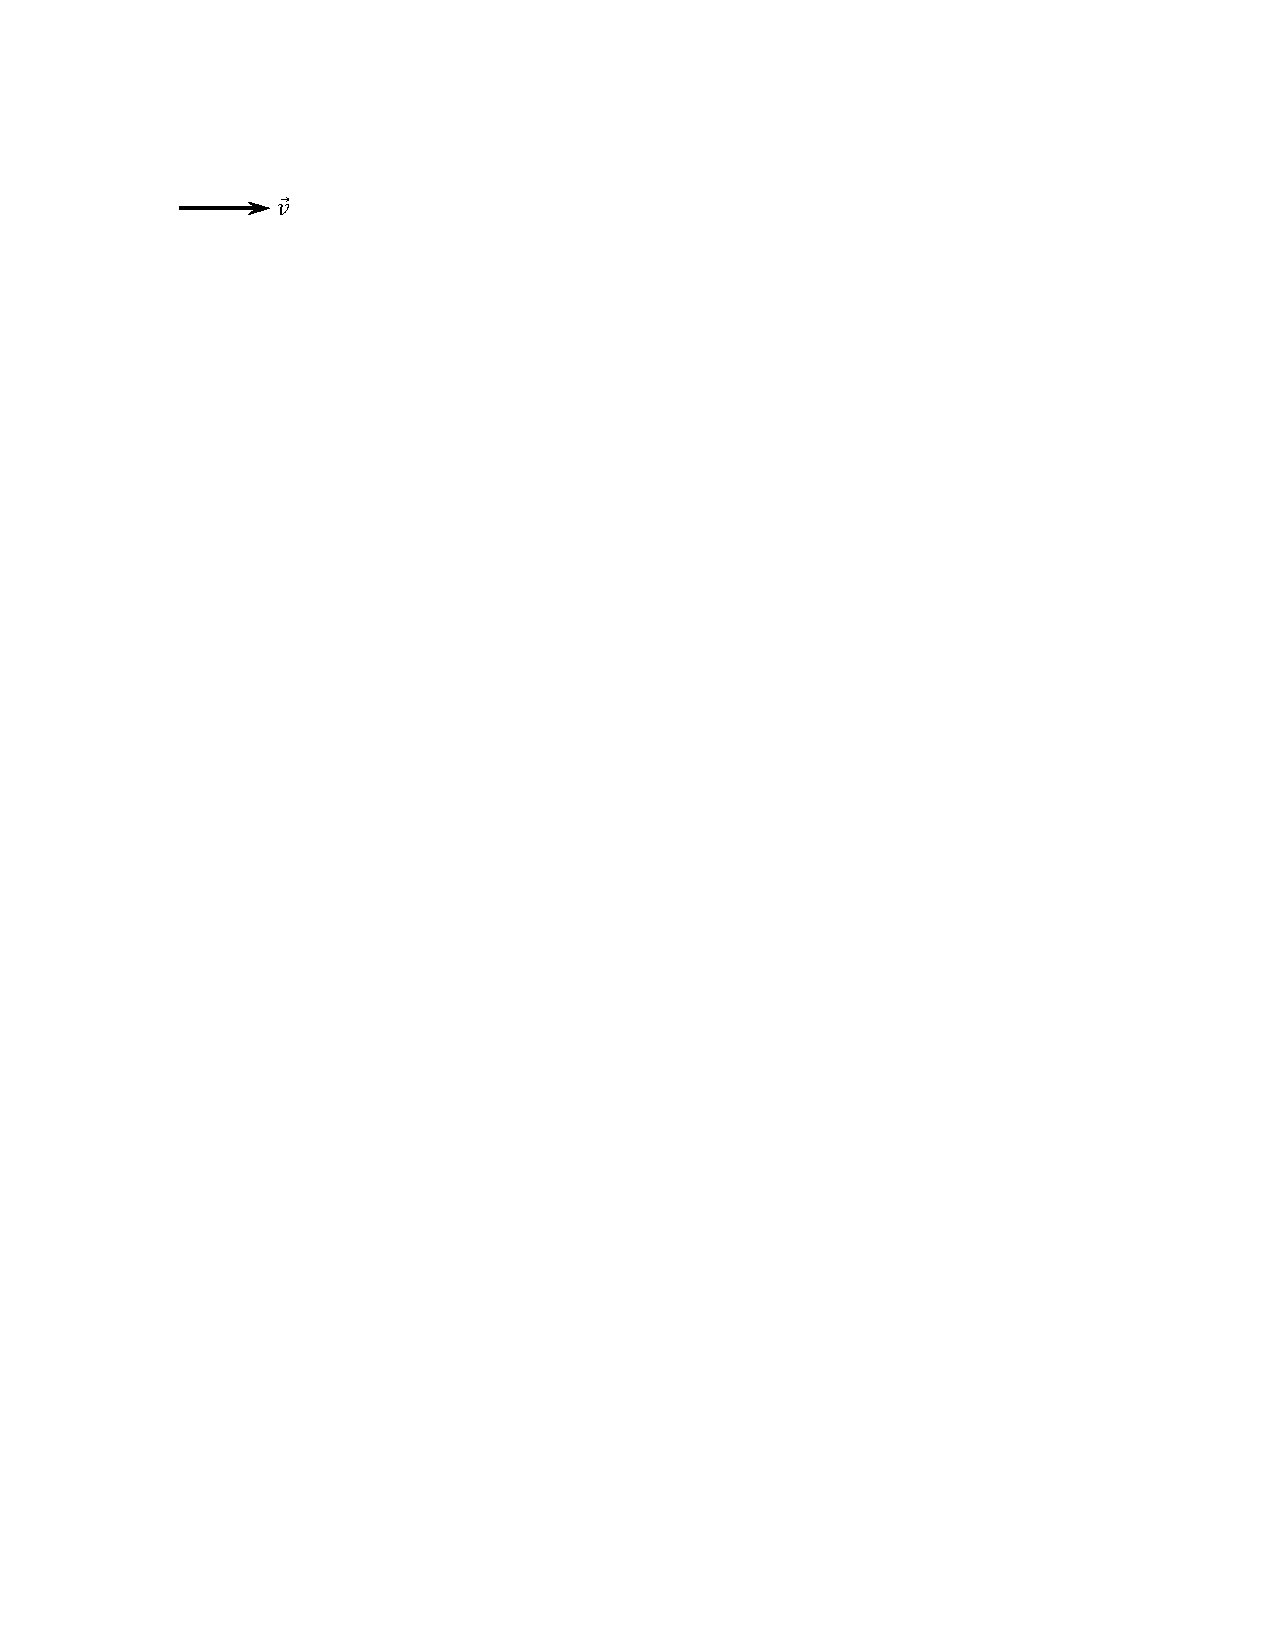
\includegraphics{velocity/velocity_vector.pdf} \par}
\vspace{0.3cm}

If you were moving twice as fast toward the right, the arrow representing your
velocity vector would look like:

\vspace{0.3cm}
%{\par\centering 
\includegraphics{velocity/velocity_fig4.eps} \par}
{\par\centering 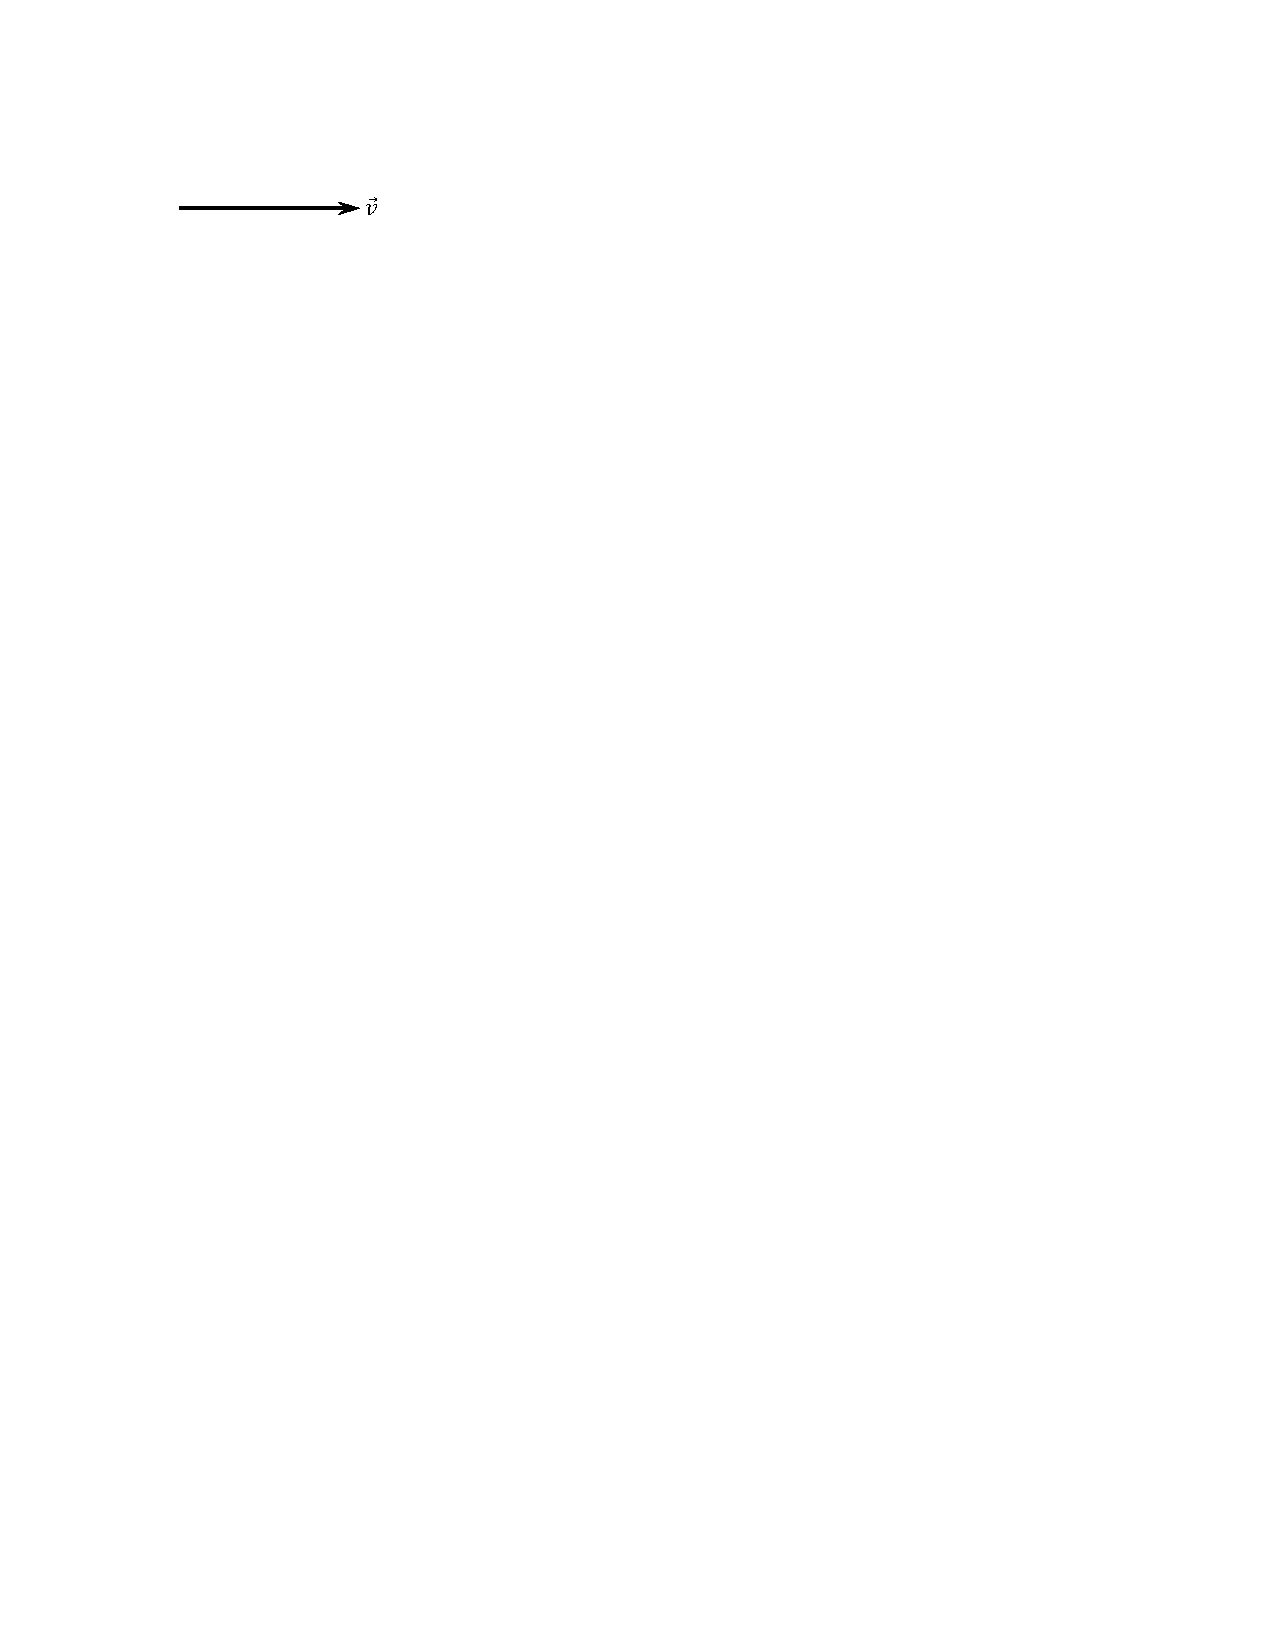
\includegraphics{velocity/velocity_vector_2x.pdf} \par}
\vspace{0.3cm}

while moving twice as fast toward the left would be represented by the following
arrow:

\vspace{0.3cm}
%{\par\centering 
\includegraphics{velocity/velocity_fig5.eps} \par}
{\par\centering 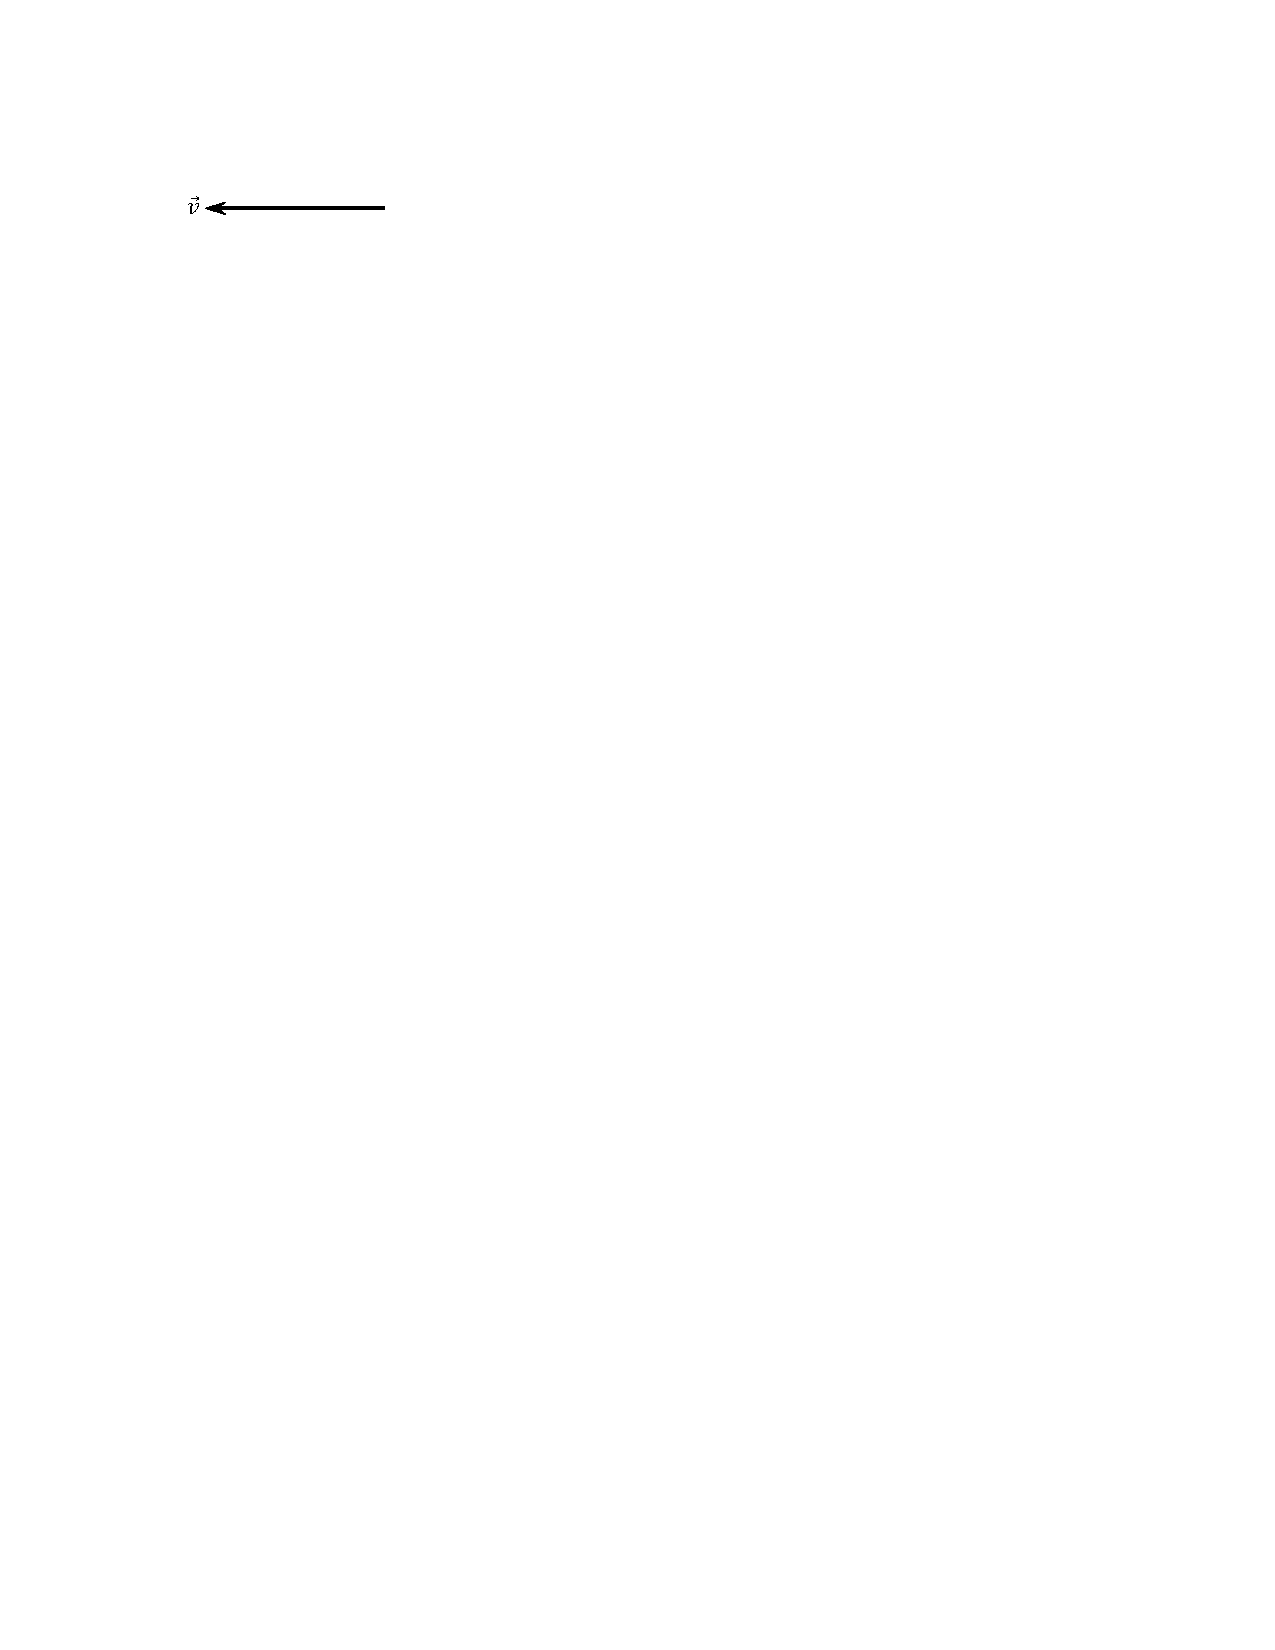
\includegraphics{velocity/velocity_vector_2x_left.pdf} \par}
\vspace{0.3cm}

What is the relationship between a one-dimensional velocity vector and the sign
of velocity? This depends on the way you choose to set the positive $x$-axis.

\vspace{0.3cm}
%{\par\centering 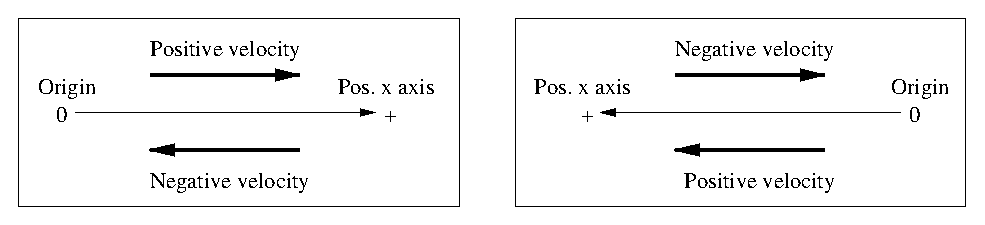
\includegraphics{velocity/velocity_fig6.eps} \par}
{\par\centering 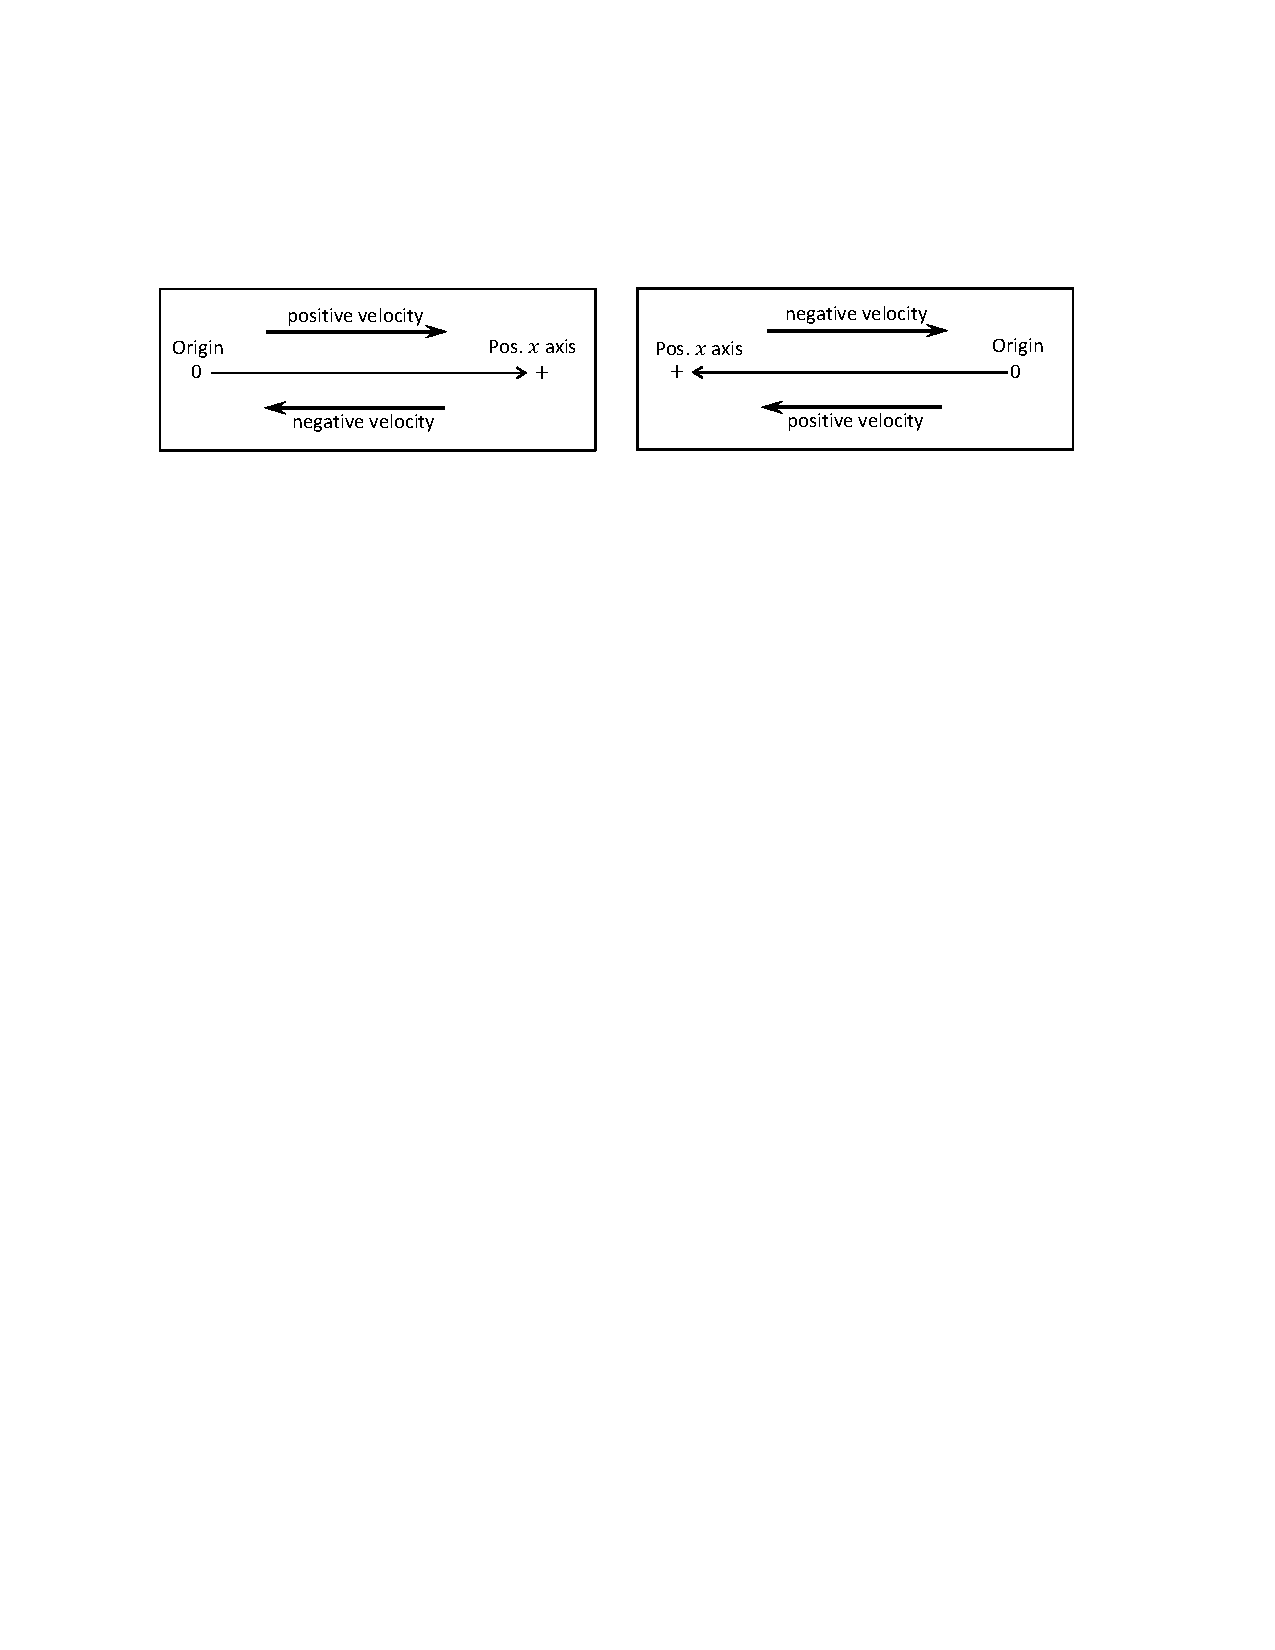
\includegraphics{velocity/velocity_signs.pdf} \par}
\vspace{0.3cm}

In both diagrams the top vectors represent velocity toward the right. In the
left diagram, the $x$-axis has been drawn so that the positive $x$-direction is
toward the right. Thus the top arrow represents positive velocity. However,
in the right diagram, the positive $x$-direction is toward the left. Thus the
top arrow represents negative velocity. Likewise, in both diagrams the bottom
arrows represent velocity toward the left. In the left diagram this is negative
velocity, and in the right diagram it is positive velocity.

\textbf{Activity 3: Sketching Velocity Vectors} 

Sketch below velocity vectors representing the three parts of the motion described
in the prediction you made in Activity 2.

(a) Walking slowly away from the sensor:
\answerspace{8mm}

(b) Standing still:
\answerspace{8mm}

(c) Walking rapidly toward the sensor:
\answerspace{8mm}

\pagebreak[2]
\textbf{Activity 4: Matching a Velocity Graph} 

(a) Describe how you think you will have to move in order to match the velocity
graph shown below.

%\vspace{0.3cm}
%{\par\centering 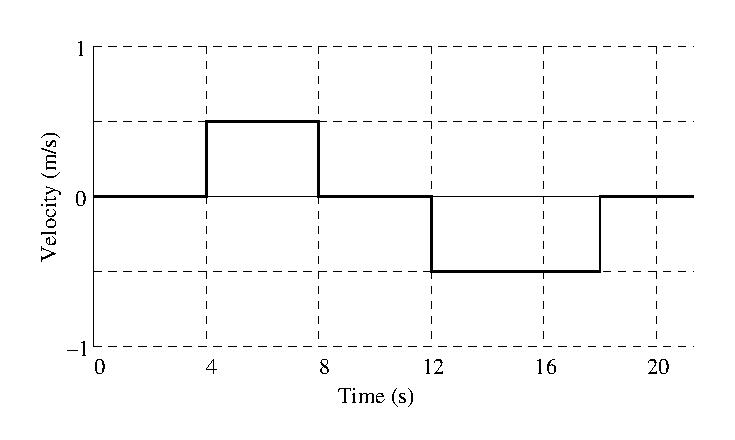
\includegraphics{velocity/velocity_fig7.eps} \par}
%\vspace{0.3cm}
\begin{lab_axis}*[lab_grid,
	width=4.5in, height=1.8in,
	xlabel={Time (s)},
	ylabel={Velocity (m/s)},
	xmin=0, xmax=20,
	ymin=-1, ymax=1,
	xtick distance = 4,
	ytick distance = 1,
	minor y tick num=1,
	minor x tick num=1,
	]
\addplot coordinates {(0,0) (4,0) (4,0.5) (8,0.5) (8,0) (12,0) (12,-0.5) (18,-0.5) (18,0) (22,0)};
\end{lab_axis}


\answerspace{25mm}
(b) Move in such a way that you can reproduce the graph shown. You may have
to practice a number of times to get the movements right. Work as a team and
plan your movements. Get the times right. Get the velocities right. You and
each person in your group should take a turn. Then sketch your group's best
match on the above graph.

(c) Is it possible for an object to move so that it produces an absolutely vertical
line on a velocity-time graph? Explain.
\answerspace{25mm}

(d) Did you run into the motion sensor on your return trip? If so, why did
this happen? How did you solve the problem? Does a velocity graph tell you where
to start? Explain.
\answerspace{25mm}

\pagebreak[2]
\textbf{Homework} 

Answer the following questions in the spaces provided.

1. How do you move to create a horizontal line in the positive part of a velocity-time
graph, as shown below?

%\vspace{0.3cm}
%{\par\raggedright 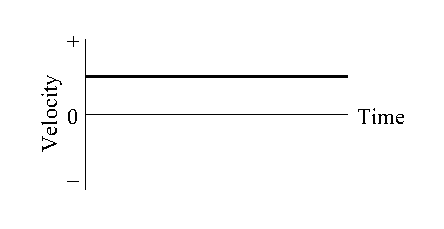
\includegraphics[width=0.45\textwidth]{velocity/velocity_fig8.eps} \par}
%\answerspace{0.3cm}
\begin{lab_axis}[lab_noticks_2quads,
	height = {1.4in}, width = {2.0in},
	xlabel={Time},
	ylabel={Velocity},
	plus_minus_zero_labels,
	]
\addplot {0.5};
\end{lab_axis}
\answerspace{0.2in}

2. How do you move to create a straight-line velocity-time graph that slopes
up from zero, as shown below?

%\vspace{0.3cm}
%{\par\raggedright 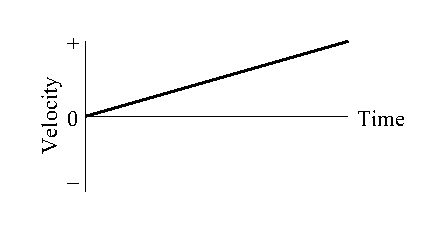
\includegraphics[width=0.45\textwidth]{velocity/velocity_fig9.eps} \par}
%\answerspace{0.3cm}
\begin{lab_axis}[lab_noticks_2quads,
	height = {1.4in}, width = {2.0in},
	xlabel={Time},
	ylabel={Velocity},
	plus_minus_zero_labels,
	]
\addplot {x};
\end{lab_axis}
\answerspace{0.2in}

3. How do you move to create a straight-line velocity-time graph that slopes
down, as shown below?

%\vspace{0.3cm}
%{\par\raggedright 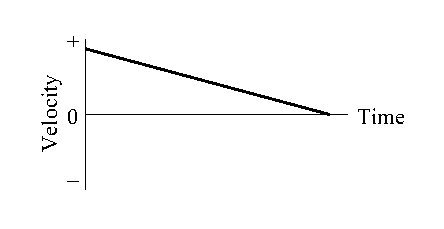
\includegraphics[width=0.45\textwidth]{velocity/velocity_fig10.eps} \par}
%\answerspace{0.3cm}
\begin{lab_axis}[lab_noticks_2quads,
	height = {1.4in}, width = {2.0in},
	xlabel={Time},
	ylabel={Velocity},
	plus_minus_zero_labels,
	]
\addplot {0.8 - 8/9*x};
\end{lab_axis}
\answerspace{0.2in}

4. How do you move to make a horizontal line in the negative part of a velocity-time
graph, as shown below?

%\vspace{0.3cm}
%{\par\raggedright 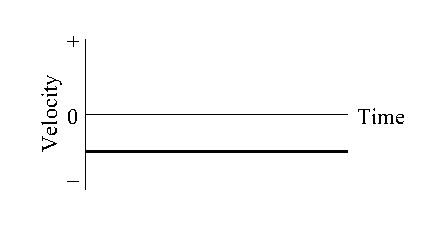
\includegraphics[width=0.45\textwidth]{velocity/velocity_fig11.eps} \par}
%\answerspace{0.3cm}
\begin{lab_axis}[lab_noticks_2quads,
	height = {1.4in}, width = {2.0in},
	xlabel={Time},
	ylabel={Velocity},
	plus_minus_zero_labels,
	]
\addplot {-0.5};
\end{lab_axis}
\answerspace{0.2in}

\pagebreak[4]
5. The velocity-time graph of an object is shown below. Figure out the total
change in position (displacement) of the object. Show your work.

Displacement = \_\_\_\_\_\_\_\_\_\_\_\_ meters.

\bigskip

%\vspace{0.3cm}
%{\par\raggedright 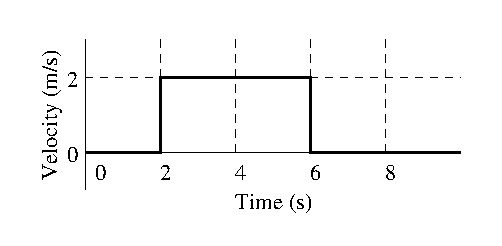
\includegraphics[width=0.55\textwidth]{velocity/velocity_fig12.eps} \par}
%\answerspace{0.6cm}
\begin{lab_axis}[lab_grid,
	height = {1.2in}, width = {3.0in},
	xlabel={Time (s)},
	ylabel={Velocity (m/s)},
	xmin=0, xmax=10,
	ymin=0, ymax=4,
	xtick distance = 2,
	ytick distance = 2,
	]
\addplot coordinates {(0,0) (2,0) (2,2) (6,2) (6,0) (10,0) };
\end{lab_axis}
\answerspace{0.1in}

6. The velocity graph below shows the motion of two objects, A and B. Answer
the following questions separately. Explain your answers when necessary. (a)
Is one faster than the other? If so,which one is faster? (A or B) (b) What does
the intersection mean? (c) Can one tell which object is ``ahead''?
(define ``ahead'') (d) Does either object A or B reverse direction?
Explain.

%\vspace{0.3cm}
%{\par\raggedright 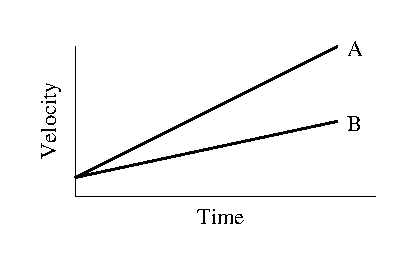
\includegraphics[width=0.45\textwidth]{velocity/velocity_fig13.eps} \par}
%\answerspace{0.6cm}
\begin{lab_axis}[lab_noticks_1quad,
	height = {1.3in}, width = {2.2in},
	xlabel={Time},
	ylabel={Velocity},
	]
\addplot coordinates {(0, 0.2) (0.9, 0.9)} node[right] {A};
\addplot coordinates {(0, 0.2) (0.9, 0.4)} node[right] {B};
\end{lab_axis}
\answerspace{0.7in}

7. The velocity graph below shows the motion of two objects, A and B. Answer
the following questions separately. Explain your answers when necessary. (a)
Is one faster than the other? If so,which one is faster? (A or B) (b) What does
the intersection mean? (c) Can one tell which object is ``ahead''?
(define ``ahead'') (d) Does either object A or B reverse direction?
Explain.

%\vspace{0.3cm}
%{\par\raggedright 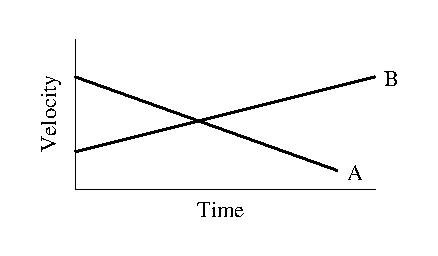
\includegraphics[width=0.45\textwidth]{velocity/velocity_fig14.eps} \par}
%\answerspace{0.6cm}
\begin{lab_axis}[lab_noticks_1quad,
	height = {1.3in}, width = {2.2in},
	xlabel={Time},
	ylabel={Velocity},
	]
\addplot coordinates {(0, 0.9) (0.7, 0.1)} node[right] {A};
\addplot coordinates {(0, 0.3) (0.9, 0.6)} node[right] {B};
\end{lab_axis}
\answerspace{0.7in}

\pagebreak[3]
An object moves along a line (the + position axis). Sketch the velocity-time graph corresponding to each of the following descriptions of its motion.

8. The object is moving away from the origin at a constant velocity.

%\vspace{0.3cm}
%{\par\centering 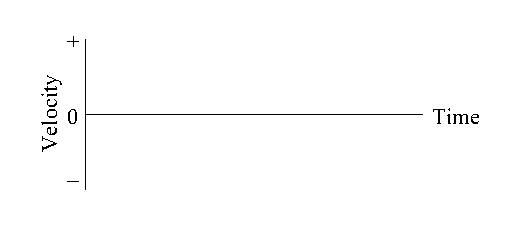
\includegraphics{velocity/velocity_fig15.eps} \par}
%\vspace{0.3cm}
\begin{lab_axis}*[lab_noticks_2quads,
	height = {1.2in}, width = {2.4in},
	xlabel={Time},
	ylabel={Velocity},
	plus_minus_zero_labels,
	]
\end{lab_axis}

9. The object is standing still.

%\vspace{0.3cm}
%{\par\centering 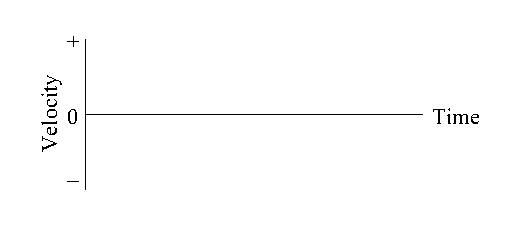
\includegraphics{velocity/velocity_fig15.eps} \par}
%\vspace{0.3cm}
\begin{lab_axis}*[lab_noticks_2quads,
	height = {1.2in}, width = {2.4in},
	xlabel={Time},
	ylabel={Velocity},
	plus_minus_zero_labels,
	]
\end{lab_axis}

10. The object moves toward the origin at a steady (constant) velocity for 10
s and then stands still for 10 s.

%\vspace{0.3cm}
%{\par\centering 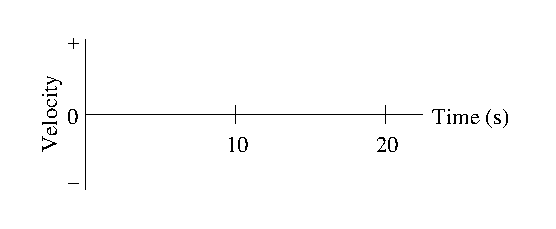
\includegraphics{velocity/velocity_fig16.eps} \par}
%\vspace{0.3cm}
\begin{lab_axis}*[lab_noticks_2quads,
	height = {1.2in}, width = {2.4in},
	xlabel={Time (s)},
	ylabel={Velocity},
	xmax=23,
	xtick={10,20},
	plus_minus_zero_labels,
	]
\end{lab_axis}


11. The object moves away from the origin at a steady (constant) velocity for
10 s, reverses direction and moves back toward the origin at the same speed
for 10 s.

%\vspace{0.3cm}
%{\par\centering 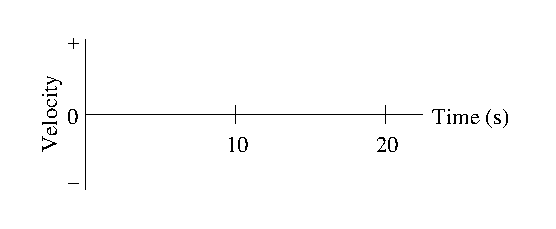
\includegraphics{velocity/velocity_fig16.eps} \par}
%\vspace{0.3cm}
\begin{lab_axis}*[lab_noticks_2quads,
	height = {1.2in}, width = {2.4in},
	xlabel={Time (s)},
	ylabel={Velocity},
	xmax=23,
	xtick={10,20},
	plus_minus_zero_labels,
	]
\end{lab_axis}


